\chapter{Background}

\label{ch:background}

\section{Workload-Aware Frameworks}

\subsection{Database Cracking}

From Idreos et al., Cracking is a relational database auto-tuning technique which performs online
restructuring of a relational table into disjoint pieces, storing information about each piece within
a separate data-structure called the cracker index.

When a column is queried, it is copied into a version of the column called the cracker column. The
cracker column is then scanned, restructuring it in-place to position the retrieved elements in
contigious positions. The indices of the bounds of the newly formed contigious region are stored
within the cracker index to inform future queries of whether they need to scan that piece of the
column.

Figure \ref{fig:cracking_img} shows two queries being run against a column within a system employing
database cracking. We can see that Q1 partitions copies the column into a cracker column, which is
then partitioned into pieces, of which information is known about the contents. Q2 further breaks
up the column into pieces, and again the information about the newly formed partitions is stored
in the cracker index.

\begin{figure}[h]
  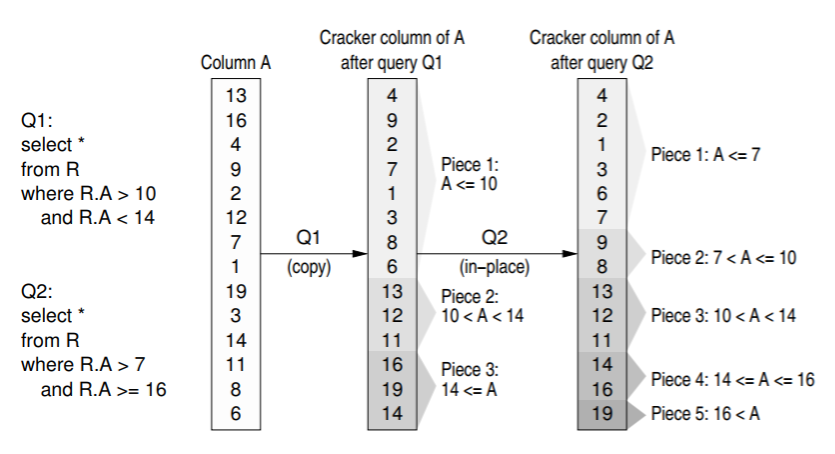
\includegraphics[width=\textwidth]{cracking_img}
  \caption{Illustration of database cracking}
  \label{fig:cracking_img}
\end{figure}

\subsubsection{Algorithm}

We will lay out in this subsection our description of the 'cracker selection in three' algorithm
in words, so that the adaptive compression chapter, which draws heavily on this work, it is easier
for readers to follow the action.

In the first stage of the algorithm, a contiguous section of the column is selected for scanning by
selecting two pointers from the cracker index, between which all of the result tuples are known to
lie. If the cracker index is empty, then the entire column is selected as the sole fragment of the
column. We will commonly refer to a section of the column which can be specified by values inside the cracker index as column fragments, or just fragments.

If \texttt{(value, index)} is stored in the cracker index, then at all indices preceeding
\texttt{index}, the corresponding value in the cracker column is strictly less than \texttt{value}.

In order to map back from the cracker column to the original columns of the table, we use an array
which is initialised to store successive integers from 0, of the same length as the table. We apply
all swapping operations to this array as well as the cracker column, which means that any range of
values in the cracker column have indices which map to those same values in the original column of
the original table. We refer to this array as the \texttt{base\_idx} array

We define two predicates with respect to the selected range of values. The first returns true when
its input is outside of the selection on the lower end, the second returns true if the input is
outside the selection on the higher end. We will refer to these predicates as lowp and highp
respectively.

The selected fragment is defined by two edge pointers which we have looked up. One pointing at the
lower side of the fragment, \texttt{low\_ptr}, and one pointing at the upper side, \texttt{high\_ptr}.
At all times during the algorithm, we will maintain the invariant that all indices before
\texttt{low\_ptr} will point to a value in the cracker column which satisfies lowp. Similarly, all
pointers after \texttt{high\_ptr} point to a value in the cracker column satisfying highp. By "all pointers", I mean all valid pointers across the entire of the cracker column.

We then tighten the two edge pointes inwards while the associated invariant holds. We will refer to
this procedure as tightening.

The next part involves scanning the fragment between the edge pointers. An iteration pointer,
\texttt{itr\_ptr}, begins at the same point as \texttt{low\_ptr}, scanning upwards. For each value that it encounters in the cracker column, it is determined using the predicates, in which region of
the column the value belongs - the low side out-of-bounds region, the selected region, or the upper
side out-of-bounds region. If the value is not selected, that is, if it's out-of-bounds, it is swapped
with the value at the respective edge pointer. The edge pointer is then tightened - resulting in it
moving inwards by at least one, since the swapped-in value was determined to be out-of-bounds on that
side. During the scan, we maintain the loop invariant that all indices before \texttt{itr\_ptr} point
to a value in the cracker column which satisfies either lowp, or is within the selected range, which
is equivalent to saying that all the indices from \texttt{low\_ptr} inclusive to \texttt{itr\_ptr}
exclusive are within the selected range. At the end of the algorithm therefore, we will find that
this corresponds with the inclusive range from \texttt{low\_ptr} to \texttt{high\_ptr}, which is
defined by lowp values earlier in the column and highp values later in the column.

After the scan is concluded, we have access to some information about the column we wish to store
within the cracker index. The value at \texttt{low\_ptr} in the cracker column exceeds the values in all preceeding indices, therefore we store the key-value pair (cracker-column[\texttt{low\_ptr}],
\texttt{low\_ptr}) to indicate this fact. Similarly, we know that all values at indices strictly greater than \texttt{high\_ptr} are strictly greater than the value stored at \texttt{high\_ptr}, so
we store (cracker-column[\texttt{high\_ptr}] + 1, \texttt{high\_ptr} + 1)\footnote{For integers, the
minimum difference between elements is 1, however, for other datatypes, this may be different. See
\ref{sss:perfragment} for a brief discussion on this point.}.

Having acquired the range of indices in which our desired range of values lies in the cracker column,
we map this back to indices of the original columns using the \texttt{base\_idx} array, collect the
values from the required columns, and return them.

\subsection{Group-by-Query}

In-part inspired by cracking was the thesis work of Aluç, who proposed a group-by-query (G-by-Q)
representation for RDF data, for which the structure of individual database records, as well as
the way records are serialized on the storage system are dynamically determined based on the
workload. This technique proved to be fast and robust against other popular frameworks for
querying RDF data, however, the system is complicated - Aluç's implementation was reported to be
over 35,000 lines of C++. In this work we are aiming to produce simpler contributions.

\section{Frequency Based Clustering}

\section{Graph Algorithms}

\subsection{Breadth First Search}

Breadth first search, or BFS, when run on a graph, involves choosing a starting node as the sole
member of a frontier, which then expands in iterations, wherein members of the frontier add their
out-neighbours which have not yet been visited to the frontier, and remove themselves. This continues
until all vertices have been visited.

There are numerous optimisations which can be made to BFS to improve performance. Storing visited
nodes in a bit-vector provides an effective speed-up, for example. More interestingly, it has been
shown by Beamer et al. that dynamically switching between push and pull iterations can greatly
improve performance on low-diameter, scale free graphs.

The most important factor for us in considering BFS is that it queries the outgoing edges of each
node just once, meaning that the performance gains to be made by an adaptive model are not realised
in the course of a run-through of the algorithm. We use this algorithm to determine what cost there
is to using our adaptive query system when the first query is run, versus a pre-processing system.

\subsection{Pagerank}

Pagerank is a famous algorithm which stores a rank for each vertex and iteratively updates the values
across the entire graph. All nodes are initialised with a rank of $\frac{1}{|V|}$. During each
iteration, each node inherits from all of its in-neighbours a contribution of their pagerank divided
by their out-degree. This value is then multiplied by a damping factor and then added to a base value
to give the updated rank. The base value is defined as $\frac{1 - d}{|V|}$.

In pagerank, every iteration considers all of the vertices and edges in the graph, and so over
an execution of many iterations, any clustering or compression will see further benefits compared to
BFS.

\section{Graph Processing Frameworks}

\subsection{Ligra}

Ligra is a lightweight graph processing framework for shared-memory multi-core machines for graph
traversal algorithms, such as pagerank and BFS. They were in part inspired by Beamer et al.'s work
with shared-memory machines, acheiving speed-up by dynamically switching between push and pull implementations of BFS based on the graph's density. Ligra takes the form of a simple API of two
routines.

